% LaTeX-Vorlage Medizintechnik Projektarbeit
% Alexander Ruppel
% veraendert von Eva Eibenberger 
% veraendert von Stephan Seitz

% %%%%%%%%%%%%%%%%%%%%%%%%%%%%%%%%%%%%%%%%%%%%%%%%%%%%%%
% Please change the title of the project work, add your name 
% and matriculation number and set the language of your project 
% report 
% %%%%%%%%%%%%%%%%%%%%%%%%%%%%%%%%%%%%%%%%%%%%%%%%%%%%%%
\documentclass[%
	a4paper, %
	12pt, %
	german, % set to english if you want to write in English
	bibtotoc %
]{scrartcl}

% Gruppe: Nummer der Projektarbeit

% Thema der Projektarbeit
\newcommand{\titel}{Titel}

% Studentenname und Matrikelnummer 
\newcommand{\erster}{Peter Pan}		% Student 1: Vorname Nachname
\newcommand{\mnreins}{1234567}		% Student 1: Matrikelnummer

\newcommand{\todo}[1]{{\color{blue}{TODO: {#1}}}} 
\newcommand{\sltn}[1]{{\color{red}{SOL: {#1}}}} 
\usepackage{xcolor}
\usepackage{enumitem}


% in header Spache einstellen!
\input{header}

\begin{document}

% LaTeX-Vorlage Medizintechnik Projektarbeit
% Wintersemster 2009/10
% Alexander Ruppel
% veraendert von Eva Eibenberger 
% veraendert von Paul Stöwer
% veraendert von Mischa Dombrowski

% %%%%%%%%%%%%%%%%%%%%%%%%%%%%%%%%%%%%%%%%%%%%%%%%%%%%%%
% Diese Datei muss NICHT veraendert werden
% %%%%%%%%%%%%%%%%%%%%%%%%%%%%%%%%%%%%%%%%%%%%%%%%%%%%%%

\begin{titlepage}

\begin{center}
Friedrich-Alexander-Universit\"at Erlangen-N\"urnberg\\
Artificial Intelligence in Biomedical Engineering\\
W3-Professur für Image Data Exploration and Analysis\\
Prof.\ B.\ Kainz\\
W3-Professur für Computational Imaging\\
Prof.\ F.\ Knoll\\


\vspace*{9em}

{\huge \textbf{\textsf{Medizintechnik II}}}\\[.3em]
{Projektarbeit}\\[.3em]
{Sommersemester 2023}\\

\vspace*{9em}

{\huge \textbf{\textsf{\titel}}}\\[.7em]
{\today}
\end{center}

\vfill% {
\begin{tabbing}
	\hspace*{5cm} \= Vorname Nachname \hspace*{4em} \= Matrikelnummer \kill
	Studierende*r:\> \erster \> \mnreins \\
%	\ifthenelse{\equal{\student}{\erster}}{\textbf{\erster} \> \textbf{\mnreins}}{\erster \> \mnreins} \\
%	\ifthenelse{\equal{\student}{\zweiter}}{\textbf{\zweiter} \> \textbf{\mnrzwei}}{\zweiter \> \mnrzwei} \\
%	\ifthenelse{\equal{\student}{\dritter}}{\textbf{\dritter} \> \textbf{\mnrdrei}}{\dritter \> \mnrdrei} \\
%	\ifthenelse{\equal{\student}{\vierter}}{\textbf{\vierter} \> \textbf{\mnrvier}}{\vierter \> \mnrvier} \\
%	\ifthenelse{\equal{\student}{\fuenfter}}{\textbf{\fuenfter} \> \textbf{\mnrfuenf}}{\fuenfter \> \mnrfuenf} \\
\end{tabbing}
%}

\end{titlepage}


% Inhaltsverzeichnis
\tableofcontents
\newpage

% Dateien, die den Text enthalten
\section{Einführung}%
\label{sec:einleitung}
\todo{Was ist MRT?}

\todo{Bilderfassung}


\todo{Vorteile und Nachteile}

\todo{Überblick über das Projekt}

\section{Methoden}
\subsection{k-Raum}

\todo{Erklärung des k-Raums durch Bezugnahme auf Gleichungen und Abbildungen}

\todo{Abbildung \ref{fig:real_imag} zeigt \dots} % Referenzieren Sie alle Abbildungen im Text!

\begin{equation}
r = \
\end{equation}
\begin{equation}
\phi = \
\end{equation}

\begin{figure}
\centering
\vspace{5cm}
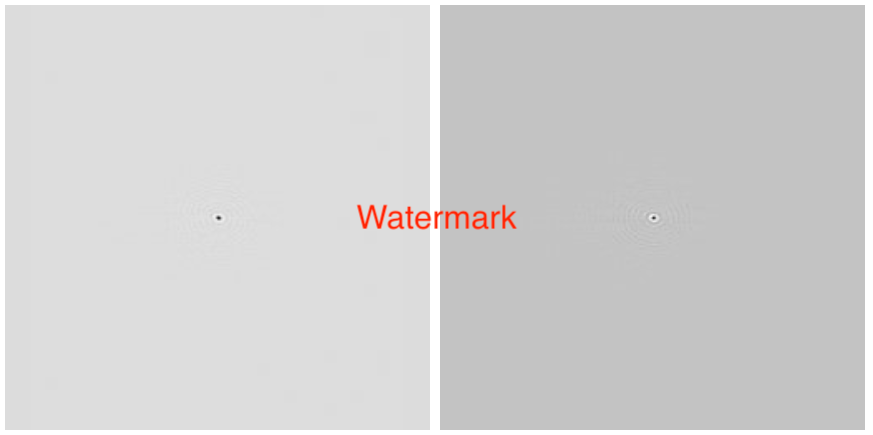
\includegraphics[width=0.6\linewidth]{latex-template-master/Grafiken/brain/realandimag.png}
\caption{\todo{Real- und Imaginärteil des k-Raums}}
\label{fig:real_imag}
\end{figure}

\begin{figure}
\centering
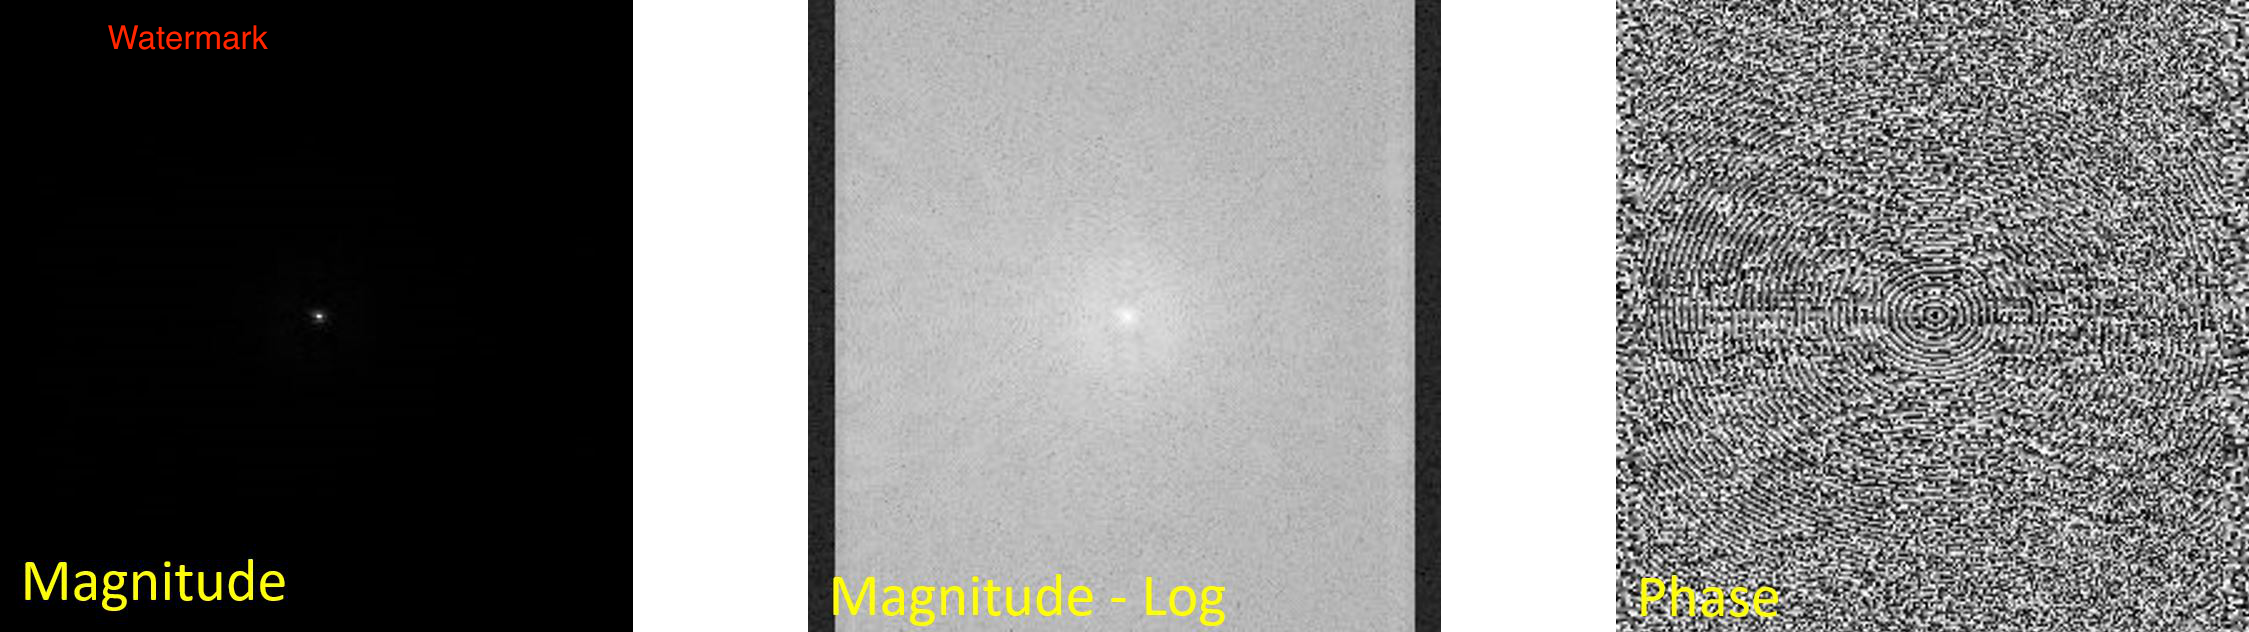
\includegraphics[width=\linewidth]{latex-template-master/Grafiken/brain/maglogphase.png}
\caption{\todo{Betrag, logarithmischer Betrag und Phase des k-Raums}}
\label{fig:mag_phas}
\end{figure}

\newpage %KANN FÜR EINREICHUNG ENTFERNT WERDEN

\subsection{Rekonstruktion}
\todo{Erklären Sie den Zweck der Rekonstruktion}

\todo{Was ist FFT-Verschiebung}

\subsubsection{Fourier-Transformation}
\todo{Erkläre Fourier-Transformation}

\subsubsection{MRI Bildrekonstruktion}
\todo{Beschreibe und interpretiere Rekonstruktion}

\todo{Was passiert, wenn wir das Verfahren der Rekonstruktion umkehren? Vergleichen Sie Abbildung \ref{fig:revert}}

\begin{figure}
\centering
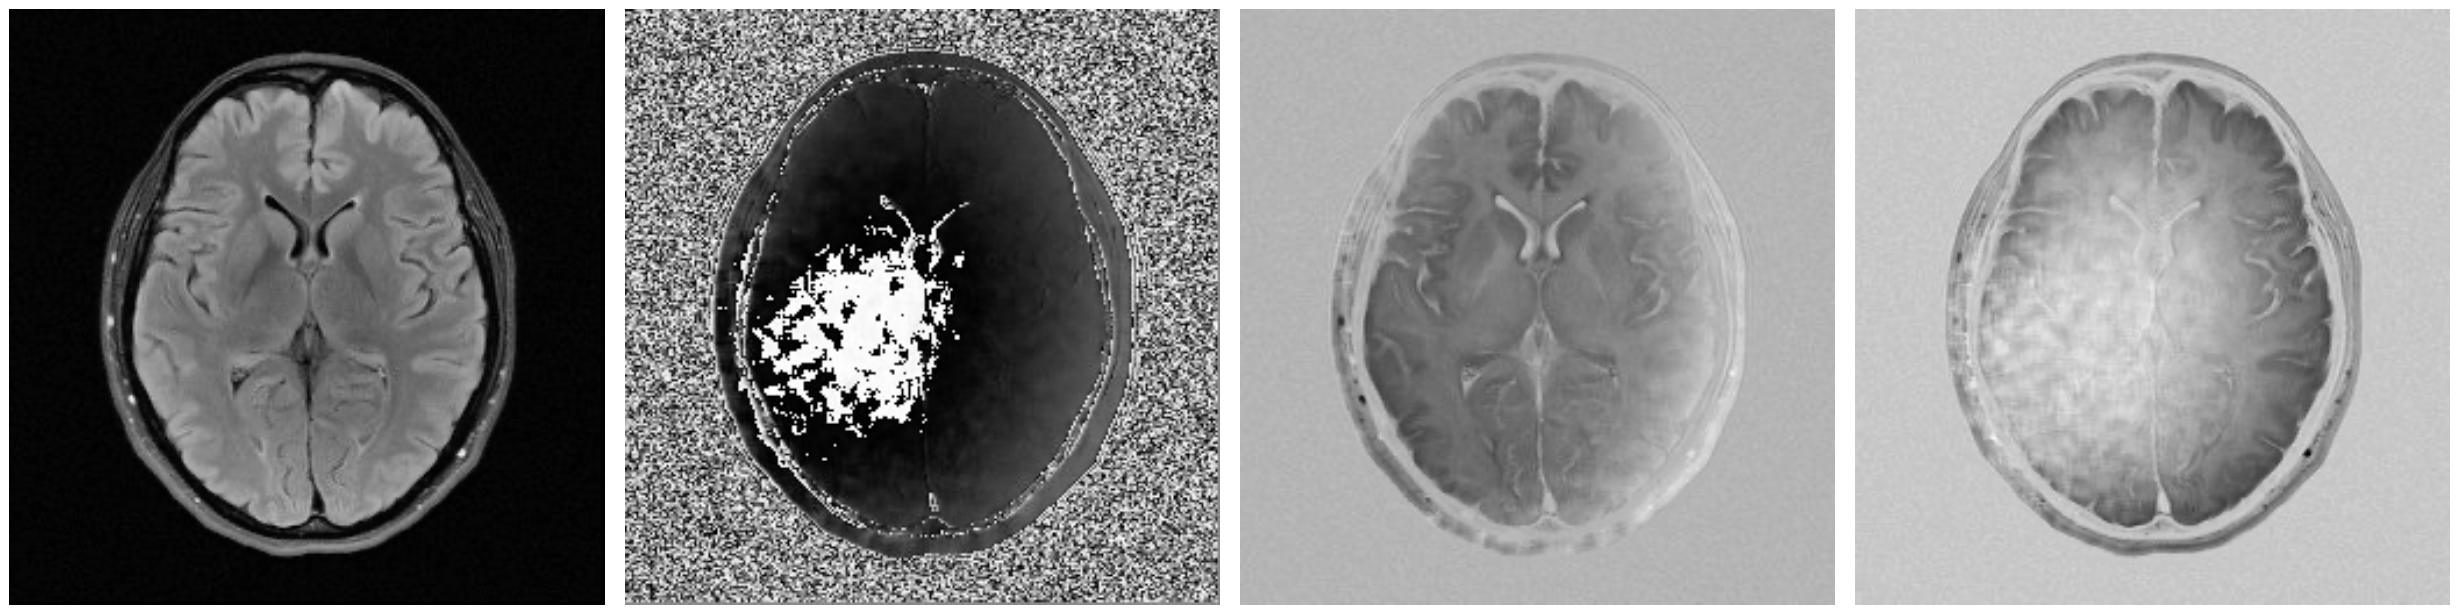
\includegraphics[width=\linewidth]{latex-template-master/Grafiken/brain/kspacereconstructed.png}
\caption{\todo{Rekonstruiertes Bild von Betrag, Phase, Real- und Imaginärteil}}
\label{fig:reconstructed}
\end{figure}

\begin{figure}
\centering
\vspace{5cm} %Platzhalter
\caption{\todo{Reproduzierte Bilder der Phase und des Betrags auf der Logarithmus-Skala}}
\label{fig:revert}
\end{figure}

\subsection{Filter}
\todo{Allgemeine Einführung in das Thema Filterung}

\subsubsection{Sinc-Filter}
\todo{Erkläre Sinc-Filterung und ihre Auswirkung}

\begin{figure}
\centering
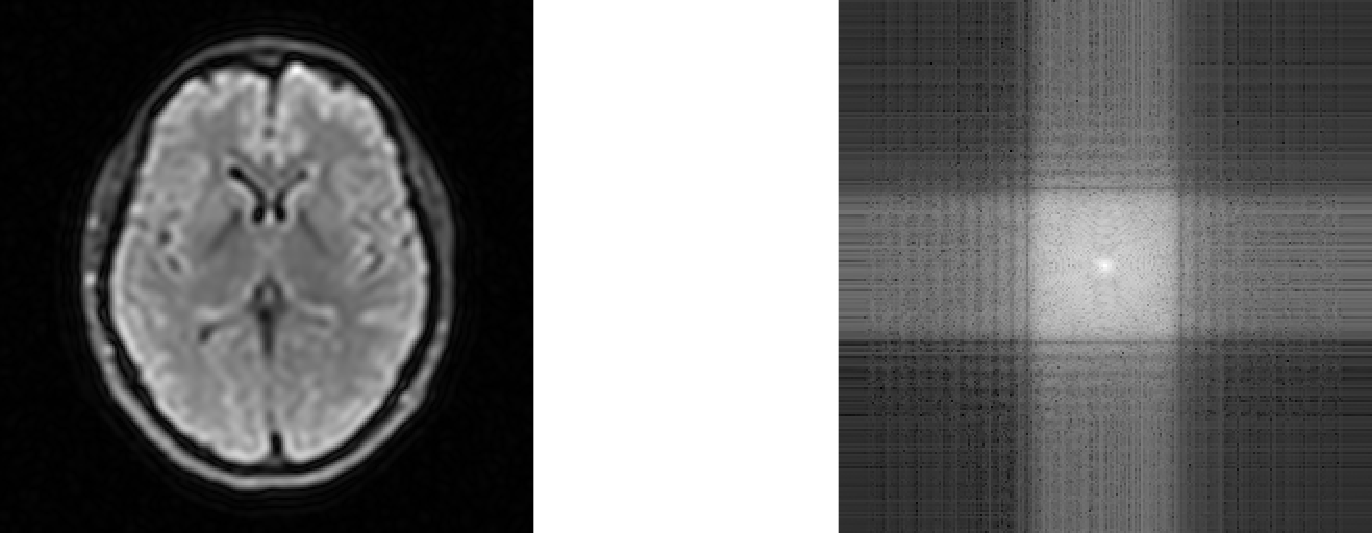
\includegraphics[width=0.9\linewidth]{latex-template-master/Grafiken/brain/sincilteredimage.png}
\caption{\todo{Die Abbildung zeigt das Betragsbild und den Betrag des k-Raums nach Anwendung der sinc-Filter.}}
\label{fig:filterungsinc}
\end{figure}

\subsubsection{Box-Multiplikation}

\todo{Erkläre die Box-Multiplikation und vergleiche sie mit dem sinc-Filter}

\todo{Erkläre die Box-Multiplikation mithilfe der Abbildung \ref{fig:kspacedifflevels}}

\begin{figure}
\centering
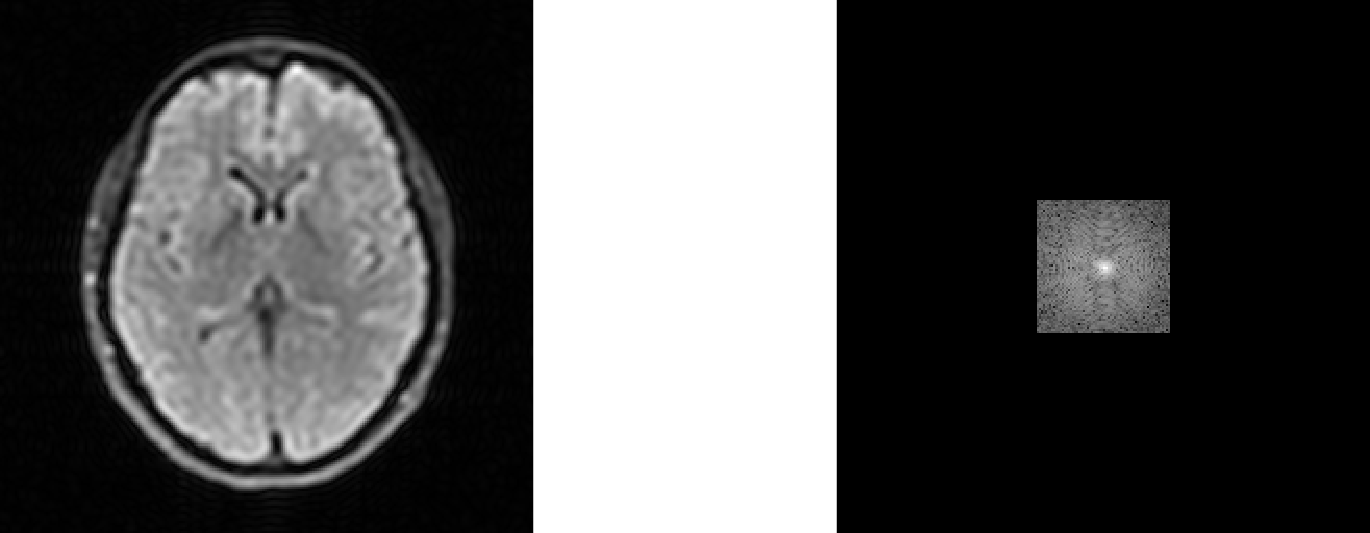
\includegraphics[width=0.9\linewidth]{latex-template-master/Grafiken/brain/boxfiltered.png}
\caption{\todo{Die Abbildung zeigt das Betragsbild und den Betrag des k-Raums nach Anwendung der Box-Multiplikation.}}
\label{fig:box-mulitplikation}
\end{figure}

\begin{figure}
\centering
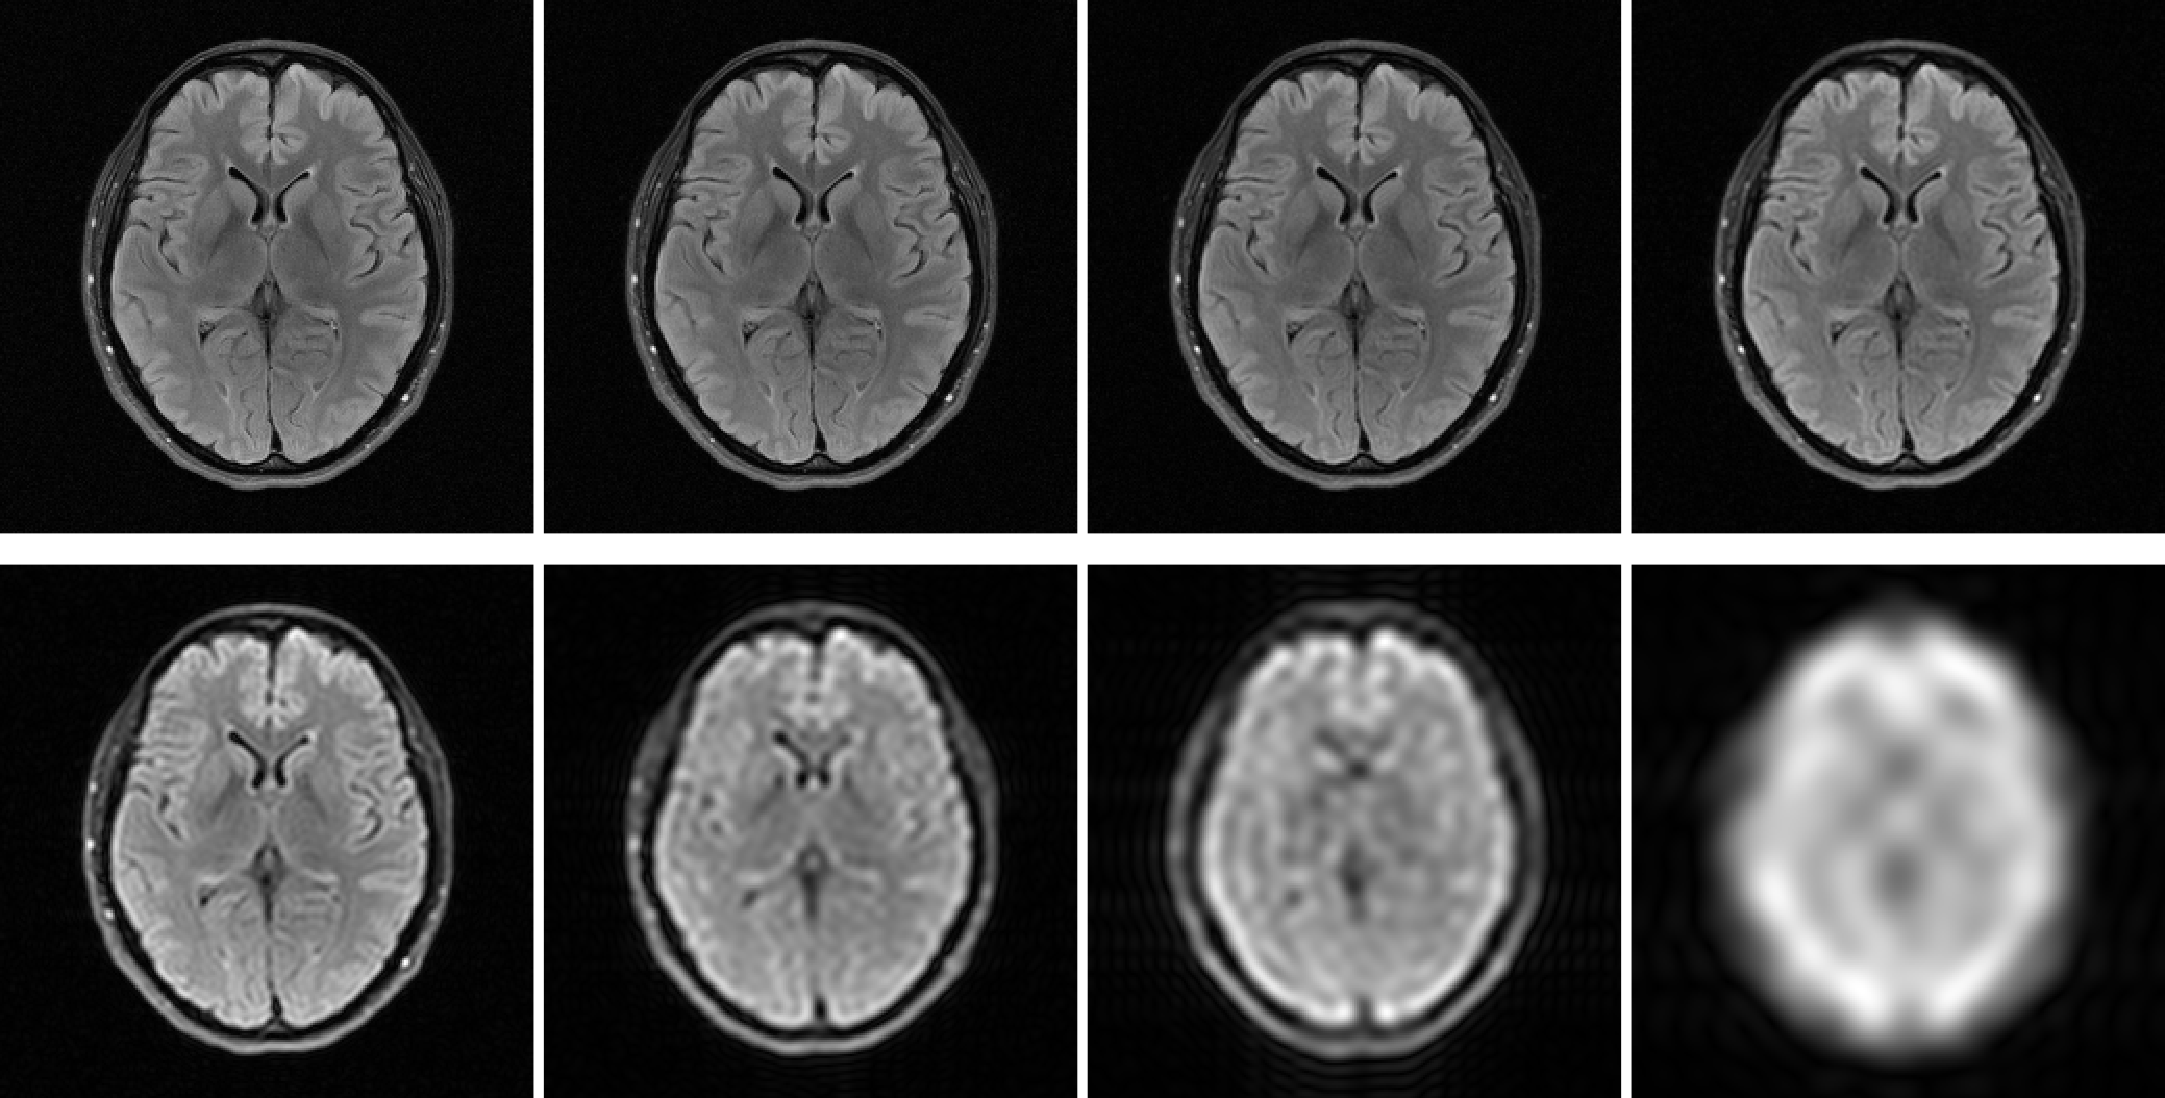
\includegraphics[width=0.9\linewidth]{latex-template-master/Grafiken/brain/kspacedifferentlevels.png}
\caption{\todo{Die Abbildung zeigt verschiedene Stufen der Bildverschlechterung durch Nullsetzung im k-Raum. TODO: Beschriften Sie die verschiedenen Stufen der nullgesetzten k-Raums.}}
\label{fig:kspacedifflevels}
\end{figure}

\newpage % TODO kann für die finale Einreichung entfernt werden

\subsection{Reduzierung der Bildgröße}

\subsubsection{Beschneiden des k-Raums}

\begin{figure}
\centering
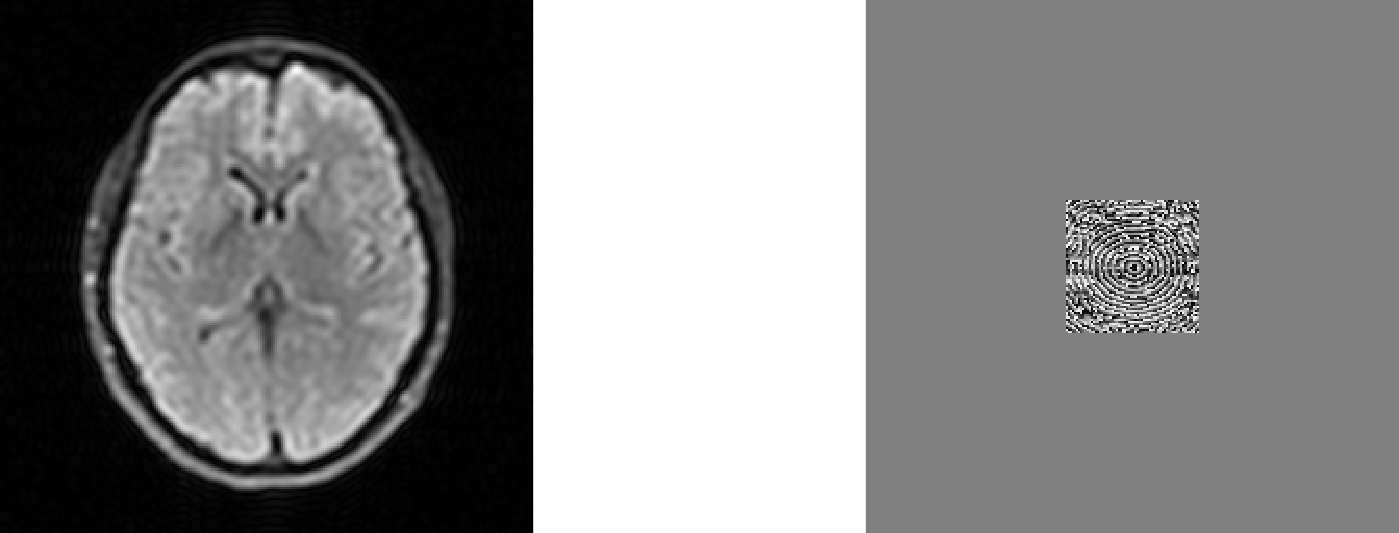
\includegraphics[width=0.9\linewidth]{latex-template-master/Grafiken/brain/croppedkspace.png}
\caption{\todo{Die Abbildung zeigt das Betragsbild und den Betrag des k-Raums nach Beschneidung im k-Raum.}}
\label{fig:kspacecrop}
\end{figure}

\todo{Erkläre das Beschneiden des k-Raums}

\subsubsection{Max-Pooling}

\begin{figure}
\centering
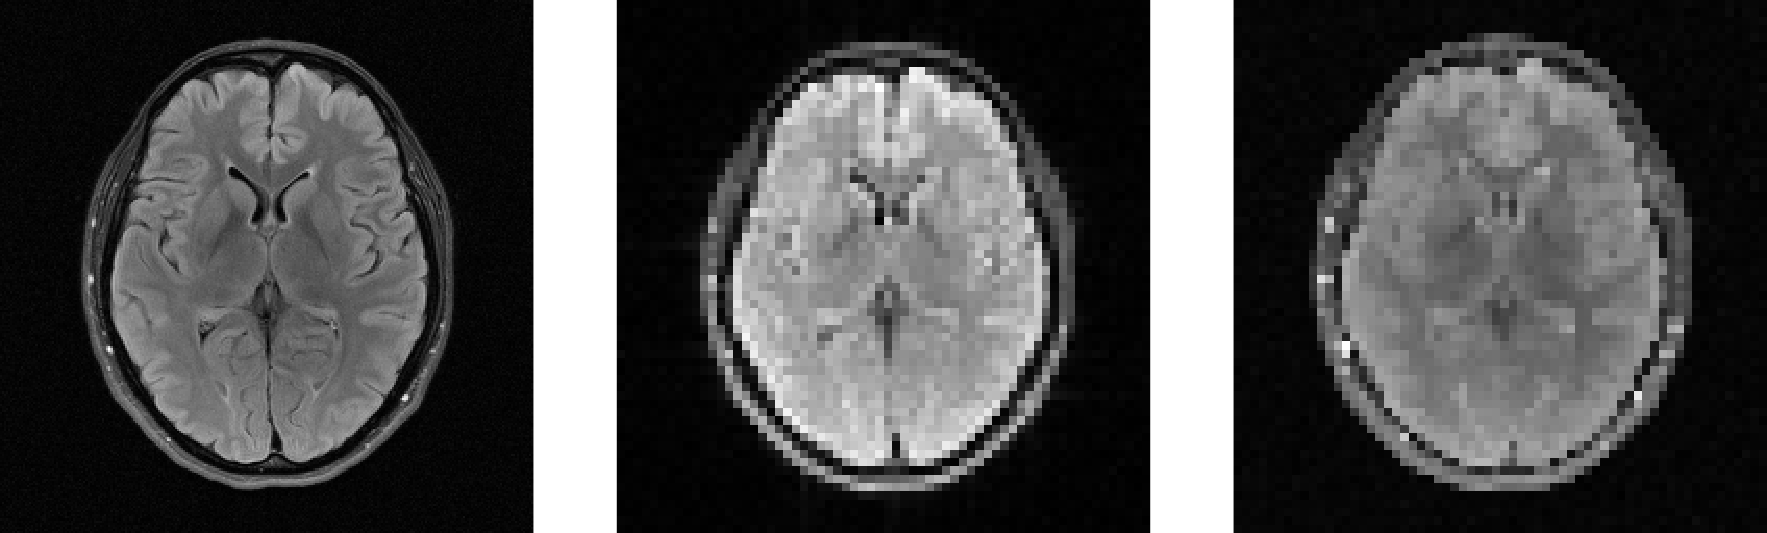
\includegraphics[width=0.9\linewidth]{latex-template-master/Grafiken/brain/maxpool.png}
\caption{\todo{Die Abbildung zeigt das Original (links), das beschnittene k-Raum-Bild (Mitte) und den Scan nach Anwendung von Max-Pooling (rechts).}}
\label{fig:maxpool}
\end{figure}

\todo{Erkläre Max-Pooling}

\todo{Vergleiche den Max-Pooling- und den beschnittenen k-Raum-Ansatz}

\section{Schlussfolgerung}

\todo{Aktuelle Forschung \cite{Jaeger09}}

% Literaturverzeichnis
\newpage
\bibliographystyle{apalike}
\bibliography{Bib/literatur}

\end{document}
  